\chapter{Background}
\label{sec:theory}

\section{Sequential decision making}

Lane keeping of a car is a sequential decision making task. Every steering action that is performed directly influences the choice of the best succeeding steering actions. \Glspl{mdp} are well suited and widely used to model sequential decision making tasks. An \gls{mdp} is a discrete time framework for a decision maker, the agent, to interact with an environment. At every time step, the environment is in a certain state, fully observable by the agent. The agent interacts with the environment by performing an action that determines the next state of the environment. The underlying assumption, the Markov property, is that the next state of the environment only depends on its current state and the agent's action. The transition to a succeeding state after an action has been performed does not need to be deterministic but can be probabilistic, accounting for randomness in the environment. After performing an action, the agent receives a numerical reward. The agent's goal is to maximize the cumulative reward it receives over time. An action that leads to a high immediate reward is not optimal if another action leads to a higher cumulative reward in the long run. Thus, the agent needs to find an optimal policy that decides the best action to take in every state. In case the state transition probabilities are known to the agent, the optimal policy can be found using model-based techniques such as value or policy iteration. If the transition model is unknown, model-free reinforcement learning can be applied to learn an optimal policy. % TODO: Add source

\begin{figure}[htbp]
    \centering
    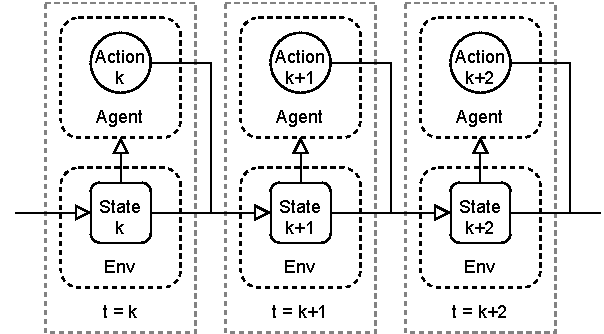
\includegraphics[width=0.75\textwidth]{figures/MDP.pdf}
    \caption{\acrfull{mdp}}
\end{figure}

Assisting a human driver in the lane keeping task is essentially a sequential decision making task as well. However, the agent that is assisting the human driver does not know about the driver's internal psychological state, and therefore her attention. A distracted driver may steer poorly and needs assistance. But how can the agent tell whether the driver is distracted? Reading the driver's mind is not feasible and even if it were, it would be too invasive for this task. Instead, the agent needs to estimate the driver's internal state in order to act adequately. A \Gls{pomdp} is a generalization of an MDP that allows to plan under uncertainty. Even without observing the full state of the agent's environment, of which the driver is part of, a POMDP allows the agent to estimate the environment's true state using the partial information it observes. A POMDP serves as the foundation of this thesis. The lane keeping assistance problem this thesis aims to solve can be defined as a POMDP. First, a formal definition is needed.

\section{Partially observable Markov decision process (POMDP)}
\label{def:pomdp}
% See POMDP Model from (POMDP algorithm) Online Planning Algorithms for POMDPs

The POMDP generalizes the MDP for planning under uncertainty. The environment's true state is unknown to the agent. It has to rely on observations with partial information about the environment's true state to choose its actions. \cite{pomdp-definition} define a POMDP as a tuple $(S, A, T, R, Z, O)$, where:
\begin{itemize}
    \item $S$ is the set of all possible states $s \in S$ of the environment. A state describes the environment at a time point. It must not be an all-encompassing description but must include all relevant information to make decisions. The state is hidden from the agent. This is the main difference to an MDP.
    \item $A$ is the set of all possible actions $a \in A$ the agent can perform in the environment.
    \item $T : S \times A \times S \rightarrow [0,1]$ defines the conditional state transition probabilities. $T(s,a,s') = Pr(s' | s, a)$ constitutes the probability of transitioning to state $s'$ after performing action $a$ in state $s$.
    \item $R : S \times A \rightarrow \R$ is the reward function providing the agent with a reward of $R(s,a)$ after performing action $a$ in state $s$.
    \item $Z$ is the set of all possible observations $z \in Z$. Observations are the agent's source of information about the environment, enabling the agent to estimate the environment's state.
    \item $O : S \times A \times Z \rightarrow [0,1]$ defines the conditional observation probabilities. $O(s', a, z) = Pr(z | s', a)$ represents the probability of receiving observation $z$ at state $s'$ after performing action $a$ in the previous state. 
\end{itemize}

At any time, the environment is in some state $s$. Unlike in the case of an MDP, the agent cannot directly observe the environment's state. Instead, the agent receives an observation $z$ that provides partial information about the current state. The agent can use the observations it perceives over time to estimate the true state of the environment and choose actions accordingly. In order to do so, at any time step $t$, it has to take into account the complete history of actions and observations until $t$:

\begin{equation}
    h_t = \{a_0,z_1,...,z_{t-1},a_{t-1},z_t\}
\end{equation}

Keeping a collection of all past observations and actions is very memory expensive. A less memory demanding alternative is to only keep a probability distribution over the states at every step, called a belief $b \in B$. $B(s,h)$ denotes the probability of being in state $s$ at time $t$ given history $h$. 

\begin{equation}
    B(s,h) = Pr(s_t=s|h_t=h)
\end{equation}

The belief is a sufficient statistic for the agent to form a decision about its next action \parencite{pomdp-belief}. Thus, only the belief needs to be kept and continually updated whenever an action is performed and a new observation arises. The agent starts with an initial belief $b_0$ about the initial state of the environment. At every subsequent time step $t$, the belief can be updated based on the previous belief $b_{t-1}$, the last action $a_t-1$ and the current observation $z_t$. The previous belief can then be discarded as the history it represents is no longer up-to-date.

% Update bayes rule
% POMCP - bayes belief rule only for small state spaces (see Monte-Carlo Belief State Updates)


Since the history that was represented by 

The agent has a belief $b$ about the state space $S$ that represents a probability distribution over the underlying states with $b(s_t)$ denoting the probability of being in state $s$. The agent acts according to its policy $\pi(b) \in A$ mapping beliefs to actions. When an action $a$ is performed, the agent receives a reward $\mathcal{R}(s,u)$ and the environment's hidden state transitions to $s' \in \mathcal{S}$ resulting in an observation $z' \in \mathcal{O}$. The agent then uses this observation to update its belief.

Solving a \gls{pomdp} consists in finding an optimal policy $\pi*$ that maximizes the belief-value function $V^\pi(b_t) = \mathbb{E}[\sum_{n=t}^{N}\lambda^{(n-t)}R(s_n,u_n)]$ that represents the cumulative reward obtained starting from initial belief $b_t$ following a policy $\pi$ over some time horizon $N$ using a discount factor $0 \leq \lambda \leq 1$.


\section{POMDP Solvers}

% Planning: Computational process that takes a model as input and produces or improves a policy for interacting with the modeled environment.
% Learning: Whereas planning methods use simulated experience generated by a model, learning methods use real experience generated by the environment.
\subsection{Offline and online solvers}

%  See: Comparison of Online POMDP and Offline POMDP - (POMDP, Thesis, DESPOT) Probabilistic Motion Planning in Uncertain and Dynamic Environments

% Generally, POMDP solver can be classified into two categories, online solver and offline solver.
% Since the traffic environments are nondeterministic and the dimension of the motion planning
% problem for autonomous driving is quite large, online solver behaves much better to duel with
% the uncertain environment and huge observation space [16].

% All these methods are offline algorithms, meaning that they
% specify, prior to the execution, the best action to execute for all possible situations. While these approximate algorithms can achieve very good performance, they often take signif-
% icant time (e.g. more than an hour) to solve large problems, where there are too many
% possible situations to enumerate (let alone plan for). Furthermore, small changes in the
% environment’s dynamics require recomputing the full policy, which may take hours or days.

\begin{figure}[htbp]
    \centering
    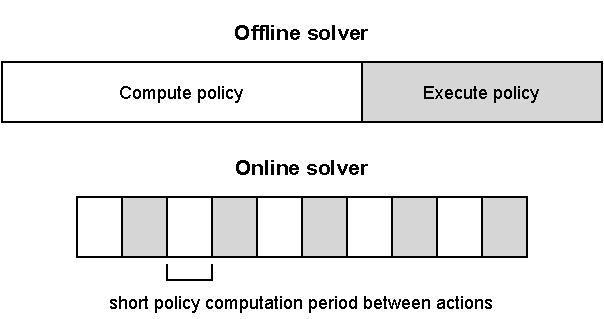
\includegraphics[width=0.75\textwidth]{figures/online-offline.pdf}
    \caption{Comparison of offline and online solving procedure}
\end{figure}

% TODO: REFINE


There are two general approaches to solve a \gls{pomdp}: offline and online. Following the offline approach, a policy depending on all possible future events is computed in advance. A policy that has been derived by offline planning can then be executed very efficiently online. However, offline planning is hard to scale to complex problems as the number of possible future events grows exponentially with the size of the planning horizon. In the online approach, planning and plan execution are intertwined. Rather than computing a policy for all possible events in advance, the belief is updated at every time step by searching for a single best action for the current belief and executing it. Then, the planning process repeats with the new belief. On the one hand, the scalability is greatly increased. On the other hand, sufficiently more complex online computation than with offline planning is required. The amount of available online planning time at each time step limits the performance. This thesis focuses on the online planning approach.

\subsection{Curse of dimensionality and curse of history}

\subsection{Monte Carlo tree search solvers}
\subsubsection{Overview}

% POMCP
% Recently an online POMDP planning algorithm called POMCP has successfully scaled up to very 
% large POMDPs [18]. POMCP, which is based on Monte Carlo tree search, tries to break the two
% curses by sampling states from the current belief and sampling histories with a black-box simula-
% tor. It uses the UCT algorithm [9] to control the exploration-exploitation trade-off during the online
% lookahead search. However, UCT is sometimes overly greedy and suffers the worst-case perfor-
% mance of Ω(exp(exp(...exp(1) ...)))1 samples to find a sufficiently good action [4].

% DESPOT
% This paper presents a new algorithm for online POMDP planning. It enjoys the same strengths
% as POMCP—breaking the two curses through sampling—but avoids POMCP’s extremely poor
% worst-case behavior by evaluating policies on a small number of sampled scenarios [13]. In each
% planning step, the algorithm searches for a good policy derived from a Determinized Sparse Par-
% tially Observable Tree (DESPOT) for the current belief, and executes the policy for one step. A
% DESPOT summarizes the execution of all policies under K sampled scenarios. It is structurally
% similar to a standard belief tree, but contains only belief nodes reachable under the K scenarios

% The general concept of online POMDP planning is that the solver computes the next optimal
% action based on the current belief state by searching in a certain depth ahead. DESPOT
% adopts this concept and improves the computational efficiency by shrinking the observation
% space.

% In order to do an efficient search in a large and deep belief tree, it is pruned and transferred 
% to Determinized Sparse Partially Observable Tree. The construction of DESPOT is sampled by the 
% K scenarios, which are shown as dots in the figure. A scenario is a determinized simulation 
% trajectory from the root of the tree. Each Q-state maintains the scenarios from its ancestor.
% And the observation is determinized by the randomly sampled scenarios. Each depth of the tree 
% can be regarded as one time-step forward simulation of the model. Thus the observation space is 
% sampled by the scenarios, but the action space is kept as its original size.





% Requirement of observation probabilities for other solvers
Other solvers have build upon the principle from POMCP of using Monte Carlo tree search for POMDP planning. 
Notably, there are DESPOT, POMCPOW, ... TODO ...
They all have an important requirement in common: The observation probabilities need to be known to the solver. Thereby, particles that are added to the belief can be weighed by how likely their associated observation is at the current belief state after performing a certain action in the prior state. However, the observation probabilities are essentially unknown in our assisted driving scenario. 

% TODO ...

\subsubsection{POMCP}
\label{sec:pomcp}

% explain: 
% - Planning versus learning
% - How POMCP breaks the curse of dimensionality with Monte-Carlo sampling
% - Belief and blief update

% Particle filter belief update:
% See (POMDP, Thesis) Tactical Decision-Making forHighway Driving

% TODO: Replace planning time with number of searches

\begin{figure}[htbp]
    \centerfloat
    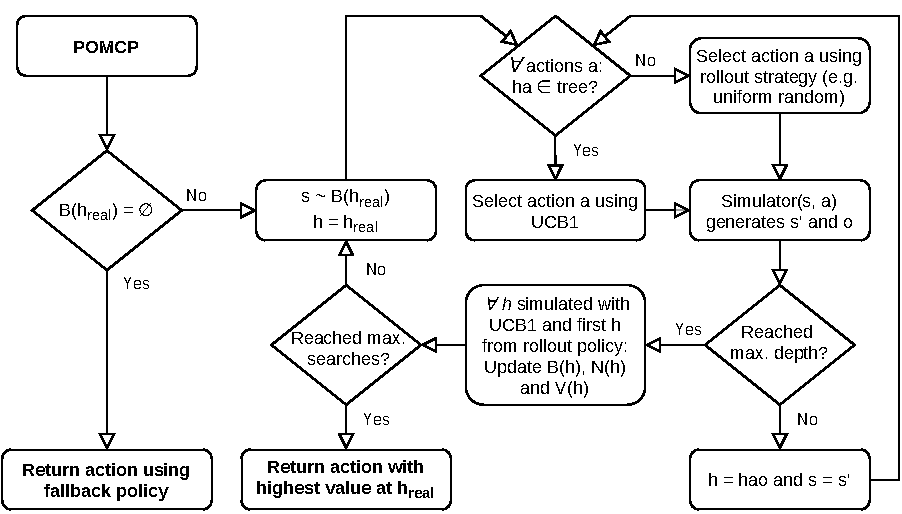
\includegraphics[width=1.2\textwidth]{figures/POMCP.pdf}
\end{figure}

\Gls{pomcp} constructs a search tree with nodes representing histories $h$ of actions and observations. At each node, $N(h)$ stores the number of times the represented history $h$ has been encountered, $V(h)$ is the node's value that is approximated by the average return of simulations starting at history $h$, and $B(h)$ represents the node's belief over the real environment's state. $B(h)$ is a collection of potential states where the likelihood of each state is given by the relative number of times it is included in the collection.

If the belief at the node representing $h_{real}$ is empty, an initial state distribution $I$ is used to sample a start state $s$ for the search. Otherwise, $B(h_{real})$ is utilized. The search tree is then searched in two stages. First, in the case that the search tree already contains child nodes for all actions at the current history, UCB1 is used for the action selection. Exploration is achieved by increasing the value of rarely-tried actions by an exploration bonus. Second, when the tree is missing a node for a potential action at the current history, a rollout policy is used to select actions. In the most simple case, this means choosing uniformly random over the action space. In either case, the selected action is executed on the start state $s$, leading to a successive state $s'$, observation $o$, and reward $r$. The process is repeated with resulting successive states until a maximum depth of the tree is reached. Afterwards, the beliefs, counts, and values are updated at all nodes for the histories resulting from the UCB1 action selection, and the node for the first history resulting from the rollout policy. The belief is updated by adding the successive states $s'$ from the simulator to the collections $B(ho)$ in the nodes. If the maximum planning time has not yet been reached, another start state is sampled and the whole process repeats. When the time runs out, the action $a_{best}$ with the highest value at the current history $h_{real}$ is returned. After this action is executed in the real environment, with an observation $o_{last}$ the tree can be pruned. Only the nodes from history $h_{real}a_{best}o_{last}$ onward stay relevant as all other histories are rendered impossible.

\section{Exploration versus exploitation} % TODO: Put somewhere else